\chapter{Results and Discussion}
This chapter reports the offline comparison for each Pillar-A component and discusses what the numbers mean for the delivered system. All results are computed on the synthetic ground-truth data described in Section~5.2, over 200 seeds and held-out learner archetypes, with bootstrap confidence intervals and Holm/Benjamini--Hochberg correction as described in Section~4.3. Each component is reported for both the initial (frozen) synthetic regime and the revised (decoupled) regime that matches the booking model, so that the transfer of a result across the redesign is visible. Throughout, the oracle is the upper-bound reference that is given the planted ground truth; it is never a deployable method. Section~6.1 covers pace calibration, Section~6.2 change detection, Section~6.3 progress projection, Section~6.4 schedule generation, and Section~6.5 discusses the results together.

\section{Pace Calibration}
Table~\ref{tab:res-cal} reports the mean recovery error of the pace estimate against the planted pace, by history-length band. The reading is deliberately honest: on this retrospective metric the structured Bayesian variants do not separate from the hierarchical-Bayesian incumbent, and the incumbent is in fact the strongest deployable method at the longest histories. The context-aware enriched-shrinkage calibrator improves on the incumbent on short histories, where its shrinkage toward a population prior helps most, but it is worse at the maximum band. This is an honest null for the structured calibrators on recovery error.

\begin{table}[htbp]
\centering
\footnotesize
\caption{Pace calibration: mean recovery error (lower is better) by history-length band, frozen regime. The oracle is the upper-bound reference.}
\label{tab:res-cal}
\begin{tabular}{l r r r}
\toprule
\textbf{Method} & \textbf{Short} & \textbf{Medium} & \textbf{Long} \\
\midrule
Oracle (reference ceiling) & 0.000 & 0.000 & 0.000 \\
Enriched-shrinkage (selected) & 0.049 & 0.049 & 0.056 \\
Hierarchical Bayesian (incumbent) & 0.079 & 0.046 & 0.026 \\
Moving average & 0.094 & 0.100 & 0.090 \\
EWMA & 0.115 & 0.124 & 0.107 \\
\bottomrule
\end{tabular}
\end{table}

The reason the enriched-shrinkage calibrator was nonetheless selected is that recovery error is not the quantity the planner acts on. The planner needs a \emph{prospective} pace estimate for the next session, especially when the learner has logged little history. On that prospective metric the enriched-shrinkage calibrator is a robust improvement over the incumbent across every band and both regimes, and the improvement survives Holm correction (Table~\ref{tab:res-cal-ctx}). It is to be noted that this is exactly the low-data regime in which a new learner's plan first needs to adapt, which is why the prospective advantage was judged to matter more than the retrospective null.

\begin{table}[htbp]
\centering
\footnotesize
\caption{Enriched-shrinkage minus hierarchical-Bayesian on the prospective context-prediction error (negative favours enriched-shrinkage), with 95\% bootstrap intervals.}
\label{tab:res-cal-ctx}
\begin{tabular}{l l l}
\toprule
\textbf{Band} & \textbf{Frozen $\Delta$ [95\% CI]} & \textbf{Decoupled $\Delta$ [95\% CI]} \\
\midrule
Short & $-0.0148$ [$-0.0168$, $-0.0127$] & $-0.0145$ [$-0.0155$, $-0.0136$] \\
Medium & $-0.0262$ [$-0.0282$, $-0.0243$] & $-0.0268$ [$-0.0277$, $-0.0258$] \\
Long & $-0.0300$ [$-0.0316$, $-0.0285$] & $-0.0307$ [$-0.0316$, $-0.0299$] \\
\bottomrule
\end{tabular}
\end{table}

\section{Change Detection}
Table~\ref{tab:res-det} reports detection latency and false-alarm rate by shift type on the frozen regime. The comparison is a robust null in the sense that no exotic detector improves on the established CUSUM and critical-slowing-down frontier. CUSUM detects fastest, at roughly one and a half sessions after a shift, at the cost of the highest false-alarm rate; the critical-slowing-down and Page-Hinkley detectors trade latency for far fewer false alarms; the exponentially weighted control chart and the Bayesian online change-point detector are markedly slower; and the ADWIN detector fails to fire at all on this data. Under the combined score that penalises both late detection and false alarms, CUSUM wins on drift shifts in both regimes and is competitive on step shifts, where Page-Hinkley edges it in the frozen regime and CUSUM regains the lead in the decoupled regime.

\begin{table}[htbp]
\centering
\footnotesize
\caption{Change detection: mean detection latency (sessions, lower is better) and false-alarm rate by shift type, frozen regime. ADWIN did not fire on this data.}
\label{tab:res-det}
\begin{tabular}{l r r r r}
\toprule
& \multicolumn{2}{c}{\textbf{Step shift}} & \multicolumn{2}{c}{\textbf{Drift shift}} \\
\cmidrule(lr){2-3}\cmidrule(lr){4-5}
\textbf{Detector} & \textbf{Latency} & \textbf{False-alarm} & \textbf{Latency} & \textbf{False-alarm} \\
\midrule
CUSUM (selected) & 1.43 & 0.312 & 1.36 & 0.296 \\
Critical slowing down & 5.16 & 0.083 & 4.10 & 0.049 \\
Page-Hinkley & 3.03 & 0.149 & 2.39 & 0.139 \\
EWMA control chart & 11.95 & 0.039 & 10.68 & 0.024 \\
Bayesian online change point & 30.59 & 0.009 & 19.43 & 0.011 \\
ADWIN & --- & 0.000 & --- & 0.000 \\
\bottomrule
\end{tabular}
\end{table}

The delivered system ships the single-arm CUSUM. Its higher false-alarm rate is acceptable here because a detected shift raises a recalibration prompt rather than triggering an automatic replan (Section~4.1): a false alarm costs the learner a dismissal, not a wrongly regenerated plan, whereas a late detection costs adaptation time. Fast detection with human confirmation is the better trade for this design.

\section{Progress Projection}
Table~\ref{tab:res-proj} reports the interval coverage and point error of the projection by history-length band, for both regimes. The point error is the same for the plain Gaussian process and the conformal method because the conformal step only rescales the interval width, not the point estimate. The headline result is a coverage failure of the raw Gaussian-process interval: against a nominal 95\%, the plain interval covers only 19\% to 49\% of the time, and the shortfall worsens as the horizon lengthens. The split-conformal correction restores coverage to between 94\% and 99\%, at the same point error. Figure~\ref{fig:res-coverage} shows the gap.

\begin{table}[htbp]
\centering
\footnotesize
\caption{Progress projection: interval coverage (nominal 0.95) and point error in days, by band. Point error is shared between the plain and conformal intervals.}
\label{tab:res-proj}
\begin{tabular}{l r r r r r}
\toprule
& \multicolumn{2}{c}{\textbf{Coverage (frozen)}} & \multicolumn{2}{c}{\textbf{Coverage (decoupled)}} & \textbf{Point error} \\
\cmidrule(lr){2-3}\cmidrule(lr){4-5}
\textbf{Band} & \textbf{Plain GP} & \textbf{Conformal} & \textbf{Plain GP} & \textbf{Conformal} & \textbf{(days, frozen)} \\
\midrule
Short & 0.438 & 0.969 & 0.494 & 0.989 & 2.15 \\
Medium & 0.291 & 0.990 & 0.277 & 0.988 & 9.45 \\
Long & 0.187 & 0.937 & 0.183 & 0.988 & 20.17 \\
\bottomrule
\end{tabular}
\end{table}

\begin{figure}[htbp]
\centering
\resizebox{0.85\linewidth}{!}{%
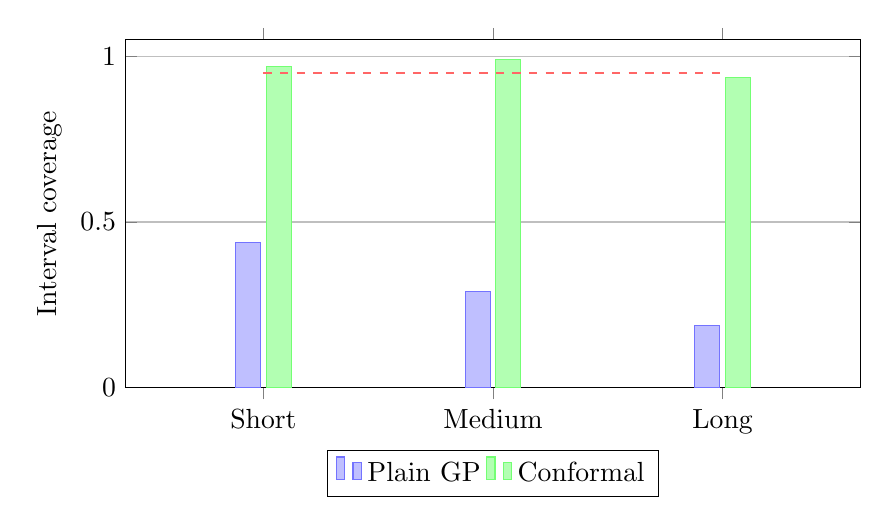
\begin{tikzpicture}
\begin{axis}[ybar, bar width=9pt, width=0.9\linewidth, height=6cm, ymin=0, ymax=1.05,
  ylabel={Interval coverage}, symbolic x coords={Short, Medium, Long}, xtick=data,
  legend style={at={(0.5,-0.18)}, anchor=north, legend columns=-1}, ymajorgrids, enlarge x limits=0.3]
\addplot[fill=blue!25, draw=blue!55] coordinates {(Short,0.438) (Medium,0.291) (Long,0.187)};
\addplot[fill=green!30, draw=green!55] coordinates {(Short,0.969) (Medium,0.990) (Long,0.937)};
\draw[dashed, thick, red!60] (axis cs:Short,0.95) -- (axis cs:Long,0.95);
\legend{Plain GP, Conformal}
\end{axis}
\end{tikzpicture}%
}
\caption{Interval coverage against the nominal 0.95 (dashed) by history-length band, frozen regime. The plain Gaussian-process interval under-covers badly; the split-conformal correction restores near-nominal coverage.}
\label{fig:res-coverage}
\end{figure}

The delivered system ships the Gaussian process with a cold-start composite that falls back to an analytic estimate when the learner has too few sessions for the process to be trusted; on the decoupled regime this composite improves cold-start coverage over the raw Gaussian process, for example lifting short-history coverage from 0.19 to 0.44. The split-conformal correction, which is the fix for the data-rich under-coverage in Table~\ref{tab:res-proj}, is validated here but is recorded as a follow-up not yet shipped; the delivered projection therefore reports an honest but under-covering interval past the cold-start threshold, a limitation returned to in Section~6.5 and Chapter~7.

\section{Schedule Generation}
Table~\ref{tab:res-sch} reports deadline drift and capacity violations by material mix on the reality-matched regime. The dynamic-programming capacity allocator minimises deadline drift in every mix, and the margin over the greedy incumbent grows sharply with the number of interleaved material roles: on the full anchor-plus-foundation-plus-practice mix the greedy incumbent drifts by roughly 39 days while the dynamic-programming allocator drifts by about 8, a difference of $-30.93$ days [$-31.70$, $-30.19$]. All candidates respect the prerequisite ordering and, apart from a negligible rate for the rule-based baseline, incur no capacity violations.

\begin{table}[htbp]
\centering
\footnotesize
\caption{Schedule generation: mean absolute deadline drift (days) by material mix, reality-matched regime. Capacity violations were zero for the selected allocator.}
\label{tab:res-sch}
\begin{tabular}{l r r r}
\toprule
\textbf{Material mix} & \textbf{DP capacity} & \textbf{Greedy incumbent} & \textbf{$\Delta$ drift [95\% CI]} \\
\midrule
Anchor & 1.73 & 3.11 & $-1.21$ [$-1.71$, $-0.72$] \\
Anchor + foundation & 2.35 & 3.65 & $-1.07$ [$-1.58$, $-0.55$] \\
Anchor + practice & 3.91 & 5.94 & $-2.03$ [$-2.71$, $-1.39$] \\
Anchor + foundation + practice & 8.30 & 38.98 & $-30.93$ [$-31.70$, $-30.19$] \\
\bottomrule
\end{tabular}
\end{table}

This is a genuine win for the dynamic-programming allocator, and it is the one component result the delivered system does not act on. As recorded in Section~4.4, the day-by-day packing formulation these schedulers share was retired during development in favour of the capacity-based booking model, because rigid packing was brittle at day boundaries and worked against continuous replanning. The scheduling comparison is therefore reported as an evaluated result that informed a design decision, not as the behaviour of the shipped scheduler.

\section{Discussion}
Read together, the results separate into honest nulls, real wins, and validated refinements not yet shipped. Calibration is a null on retrospective recovery error and a real, Holm-surviving win for the enriched-shrinkage calibrator on the prospective, short-history regime the planner actually depends on. Detection is a robust null: nothing beats the CUSUM frontier, and the shipped CUSUM is the fastest detector, which suits a human-confirmed prompt. Projection produces the clearest finding of the chapter, that the raw Gaussian-process interval under-covers severely and that a split-conformal correction fixes it; the correction is validated but deferred, so interval calibration past the cold-start threshold is a known limitation. Scheduling is a real win for a method the system deliberately does not ship, because the problem it solved was removed by the redesign.

Two cross-cutting points support the credibility of these results. First, the selected models transfer across the two synthetic regimes: the enriched-shrinkage advantage on prospective error and the projection coverage failure both hold from the frozen regime to the decoupled regime that matches the booking model, so the findings are not artefacts of one data-generating process. Second, all of this rests on synthetic data with known ground truth; the synthetic setting is what makes latency, coverage, and recovery measurable at all, but it is not a substitute for real use. Validation on a single learner's own logged sessions is deferred to Phase~II, as set out in Chapter~7.
